\documentclass[11pt]{article}
\usepackage{amsmath}
\usepackage{amssymb}
\usepackage{minted}
\usepackage{graphicx}
\usepackage{bbm}
\usepackage{float}
\usepackage[margin=0.5in,footskip=0.25in]{geometry}
\usepackage{subcaption}

\setlength{\textwidth}{6.5in}
\setlength{\oddsidemargin}{0.0in}
\setlength{\textheight}{9.0in}
\setlength{\parindent}{0in}

\def\pp{\par\noindent}
\DeclareMathOperator{\E}{\mathbb{E}}
\begin{document}

\centerline{\{\bf Amy Qi, xq2224\}}
\centerline{\bf Homework 5 Solutions}
\centerline{\bf W4771 Machine Learning --- Fall 2023}

\bigskip 
\bigskip

\section*{Problem 1}
\subsection*{(a)}
The training error rate is 0.2025. \\
The test error rate is 0.20925000000000005. \\
The final parameter matrix is 
\begin{equation}
    W = \begin{bmatrix}
        -15.56255001 & 7.98591001 & 7.57664 \\
        6.386991 & -5.62208406 & -0.76490694 \\
        3.53435652 & -0.96013681 & -2.57421971
    \end{bmatrix}
\end{equation}

\subsection*{(b)}
The graph of the negative log likelihood is a smooth curve where the value constantly decreases, whereas the graph of the error rate contains some glitches, meaning that the error rate is not always decreasing. That makes sense since we implement the gradient descent in order to minimize negative log likelihood instead of error rate.
\begin{figure}[h]
    \centering
    \begin{subfigure}{.4\textwidth}
      \centering
      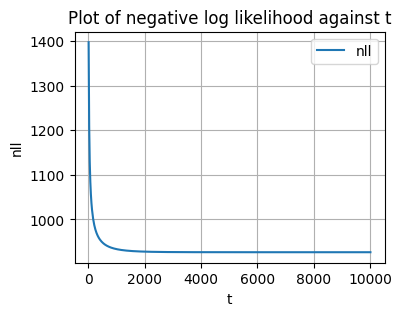
\includegraphics[width=.9\linewidth]{images/output_12_0.png}
    \end{subfigure}
    \begin{subfigure}{.4\textwidth}
      \centering
      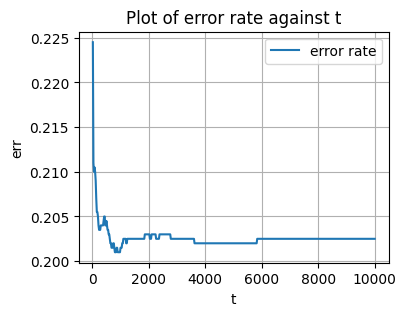
\includegraphics[width=.9\linewidth]{images/output_13_0.png}
    \end{subfigure}
\end{figure}

\newpage
\section*{Problem 2}
% \begin{equation}
%     J(w) = \frac{1}{2}w_1^2 + ln(1+exp(2w_1+w_2)) - (2w_1+w_2) +ln(1+exp(-2w_1+w_2)))
% \end{equation}
\subsection*{(a)}
This function is convex. \\

Justification: \\
To show that the function is convex, we show that each of the expressions $\frac{1}{2}w_1^2$, $ln(1+exp(2w_1+w_2))$, $-(2w_1+w_2)$ and $ln(1+exp(-2w_1+w_2))$ is convex. Since the sum of several convex function is convex, the function is convex. \\

First we show that $f_1(x) = \frac{1}{2}w_1^2$ is convex. \\
For all $u$, $v$ and all choices of $\alpha \in [0,1]$, we have 
\begin{equation}
    \begin{split}
        & f_1((1-\alpha) u + \alpha v) - [(1-\alpha) f_1(u) + \alpha f_1(v)] \\
        &= \frac{1}{2}((1-\alpha) u + \alpha v)^2 - \frac{1}{2}[(1-\alpha) u^2 + \alpha v^2] \\
        &= \frac{1}{2} \alpha (\alpha - 1) (u-v)^2
        \leq 0
    \end{split}
\end{equation}
Therefore, $f_1((1-\alpha) u + \alpha v) \leq (1-\alpha) f_1(u) + \alpha f_1(v)$, and $f_1(x)$ is convex.\\

Then we show that $f_2(x) = ln(1+exp(x))$ is convex. \\
Note that $f_2(x)$ is twice differentiable, and its second order derivative $f''(x)=(e^{-x}+1)^{-2}\cdot e^{-x} \geq 0$ holds for any $x$. Therefore $f_2(x)$ is convex. \\
Since $f_2(x)$ is convex, and both $2w_1+w_2$ and $-2w_1+w_2$ are affine functions for $w$, we know that $ln(1+exp(2w_1+w_2))$ and $ln(1+exp(-2w_1+w_2))$ are convex. \\

Finally we show that $f_3(x) = -x$ is convex. 
For all $u$, $v$ and all choices of $\alpha \in [0,1]$, we have 
\begin{equation}
        f_3((1-\alpha) u + \alpha v) - [(1-\alpha) f_2(u) + \alpha f_2(v)] = 0
\end{equation}
Therefore, $f_3((1-\alpha) u + \alpha v) \leq (1-\alpha) f_3(u) + \alpha f_3(v)$, and $f_3(x)$ is convex. Since $2w_1+w_2$ is an affine function for $w$, we know $-(2w_1+w_2)$ is convex. \\

Combining the four convex functions and we know that $J(w)$ is convex.

\subsection*{(b)}
First calculate the partial derivative with respect to $w_1$.
\begin{equation}
    \begin{split}
        \frac{\partial J(w_1, w_2)}{\partial w_1} &= w_1 + \frac{\partial}{\partial w_1} \ln(1+\exp(2w_1+w_2)) - 2 + \frac{\partial}{\partial w_1} \ln(1+\exp(-2w_1+w_2))  \\
        &= w_1 + \frac{\exp(2w_1+w_2)}{1+\exp(2w_1+w_2)} \times 2 - 2 + \frac{\exp(-2w_1+w_2)}{1+\exp(-2w_1+w_2)} \times (-2) \\
       &= w_1 - \frac{2}{1+\exp(2w_1+w_2)} - \frac{2}{1+\exp(2w_1-w_2)}
    \end{split}
\end{equation}
Then calculate the partial derivative with respect to $w_2$.
\begin{equation}
    \begin{split}
        \frac{\partial J(w_1, w_2)}{\partial w_2} &=  \frac{\partial}{\partial w_2} \ln(1+\exp(2w_1+w_2)) - 1 + \frac{\partial}{\partial w_2} \ln(1+\exp(-2w_1+w_2))  \\
        &= \frac{\exp(2w_1+w_2)}{1+\exp(2w_1+w_2)} - 1 + \frac{\exp(-2w_1+w_2)}{1+\exp(-2w_1+w_2)} \\
       &= \frac{-1}{1+\exp(2w_1+w_2)} + \frac{1}{1+\exp(2w_1-w_2)}
    \end{split}
\end{equation}
So a formula for the gradient of $J$ is
\begin{equation}
    \nabla J =
    \begin{bmatrix}
        \frac{\partial}{\partial w_1} \\
        \frac{\partial}{\partial w_2}
    \end{bmatrix} =
    \begin{bmatrix}
        w_1 - \frac{2}{1+\exp(2w_1+w_2)} - \frac{2}{1+\exp(2w_1-w_2)} \\
        \frac{-1}{1+\exp(2w_1+w_2)} + \frac{1}{1+\exp(2w_1-w_2)}
    \end{bmatrix}
\end{equation}

\newpage
\section*{Problem 3}
% \begin{equation}
%     J(w) = (logistic(2w_1+w_2)-1)^2 + (logistic(-2w_1+w_2)-0)^2
% \end{equation}
\subsection*{(a)}
This function is NOT convex. \\

If the function is convex, for all $u$, $v$ and all choices of $\alpha \in [0,1]$, $J((1-\alpha) u + \alpha v) \leq (1-\alpha) J(u) + \alpha J(v)$. However, consider the choice of $u=[-1,0],v=[0,0] \text{ and } \alpha = \frac{1}{2}$.

\begin{equation}
    \begin{split}
        J((1-\alpha) u + \alpha v) 
        &= J([-1/2, 0]) \\
        &= (logistic(-1)-1)^2 + (logistic(1))^2 \\
        &= 2 \times (logistic(1))^2 \approx 1.07
    \end{split}
\end{equation}

\begin{equation}
    \begin{split}
        (1-\alpha) J(u) + \alpha J(v) 
        &= \frac{1}{2}J([-1,0]) + \frac{1}{2}J([0,0]) \\
        &= \frac{1}{2}[(logistic(-2)-1)^2 + (logistic(2))^2 + (logistic(0)-1)^2 + (logistic(0))^2] \\
        &= (logistic(2))^2 + (logistic(0))^2 \approx 1.03 < 1.07
    \end{split}
\end{equation}

Thus we know that with choice $u=[-1,0],v=[0,0] \text{ and } \alpha = \frac{1}{2}$, $J((1-\alpha) u + \alpha v) > (1-\alpha) J(u) + \alpha J(v)$. Therefore the function is not convex.

\subsection*{(b)}
First simplify $J$ to make our lives easier.
\begin{equation}
    \begin{split}
        J(w) &= (logistic(2w_1+w_2)-1)^2 + (logistic(-2w_1+w_2)-0)^2 \\
        &= (1+e^{2w_1+w_2})^{-2} + (1+e^{2w_1-w_2})^{-2} 
    \end{split}
\end{equation}

Then calculate the partial derivative with respect to $w_1$.
\begin{equation}
    \begin{split}
        \frac{\partial J}{\partial w_1} 
        &= -2 (1+e^{2w_1+w_2})^{-3} \times \frac{\partial}{\partial w_1} (1+e^{2w_1+w_2}) - 2 (1+e^{2w_1-w_2})^{-3} \times \frac{\partial}{\partial w_1} (1+e^{2w_1-w_2}) \\
        &= -2 (1+e^{2w_1+w_2})^{-3} e^{2w_1+w_2} \times \frac{\partial}{\partial w_1} (2w_1+w_2) - 2(1+e^{2w_1-w_2})^{-3} e^{2w_1-w_2} \times \frac{\partial}{\partial w_1} (2w_1-w_2) \\
        &= -4 (1+e^{2w_1+w_2})^{-3} e^{2w_1+w_2} - 4(1+e^{2w_1-w_2})^{-3} e^{2w_1-w_2}
    \end{split}
\end{equation}

And calculate the partial derivative with respect to $w_2$.
\begin{equation}
    \begin{split}
        \frac{\partial J}{\partial w_1} 
        &= -2 (1+e^{2w_1+w_2})^{-3} \times \frac{\partial}{\partial w_2} (1+e^{2w_1+w_2}) - 2 (1+e^{2w_1-w_2})^{-3} \times \frac{\partial}{\partial w_2} (1+e^{2w_1-w_2}) \\
        &= -2 (1+e^{2w_1+w_2})^{-3} e^{2w_1+w_2} \times \frac{\partial}{\partial w_2} (2w_1+w_2) - 2(1+e^{2w_1-w_2})^{-3} e^{2w_1-w_2} \times \frac{\partial}{\partial w_2} (2w_1-w_2) \\
        &= -2 (1+e^{2w_1+w_2})^{-3} e^{2w_1+w_2} + 2(1+e^{2w_1-w_2})^{-3} e^{2w_1-w_2}
    \end{split}
\end{equation}

So a formula for the gradient of $J$ is
\begin{equation}
    \nabla J =
    \begin{bmatrix}
        \frac{\partial}{\partial w_1} \\
        \frac{\partial}{\partial w_2}
    \end{bmatrix} =
    \begin{bmatrix}
        -4 (1+e^{2w_1+w_2})^{-3} e^{2w_1+w_2} - 4(1+e^{2w_1-w_2})^{-3} e^{2w_1-w_2} \\ -2 (1+e^{2w_1+w_2})^{-3} e^{2w_1+w_2} + 2(1+e^{2w_1-w_2})^{-3} e^{2w_1-w_2}
    \end{bmatrix}
\end{equation}

\newpage
\section*{Problem 4}
\subsection*{(a)}
This function is convex. \\

Justification: \\
First we show that the function $f(x) = 1-x$ is convex.\\
For all $u$, $v$ and all choices of $\alpha \in [0,1]$, we have 
\begin{equation}
        f((1-\alpha) u + \alpha v) - [(1-\alpha) f(u) + \alpha f(v)] = 0
\end{equation}
Therefore, $f((1-\alpha) u + \alpha v) \leq (1-\alpha) f(u) + \alpha f(v)$, and $f(x)=1-x$ is convex. Since $2w_1+w_2$ is an affine function for $w$, we know $1-(2w_1+w_2)$ is convex. \\
It is easy to know that the function $g(x)=0$ is convex. \\
Since we know that if both $J_1$ and $J_2$ are convex, then $J=max\{J_1, J_2\}$ is also convex, we know that the function $J(w)=max\{0, 1-(2w_1+w_2)\}$ is convex.

\subsection*{(b)}
The affine function can be $A(w)=1-(2w_1+w_2)$. \\

Justification:\\
Substitute $u=(0,1/2)$ we know $J(u)=1/2=A(u)$. By definition, since $J(w)=max\{0, 1-(2w_1+w_2)\}$, we know that for all $w \in \mathbb{R}^2$, $J(w)\geq A(w)$.

\subsection*{(c)}
The affine function can be $A(w)=1-(2w_1+w_2)$.

Justification:\\
Substitute $u=(1/4,1/2)$ we know $J(u)=0=A(u)$. By definition, since $J(w)=max\{0, 1-(2w_1+w_2)\}$, we know that for all $w \in \mathbb{R}^2$, $J(w)\geq A(w)$.

\newpage
\section*{Problem 5}
The Frobenius norm difference is $1.4582081031998637e-13$.
\begin{equation}
    W_{\text{torch}} = \begin{bmatrix}
        -15.5626 & 7.9859 & 7.5766 \\
        6.3870 & -5.6221 & -0.7649 \\
        3.5344 & -0.9601 & -2.5742
    \end{bmatrix}
\end{equation}

\section*{Problem 6}
\subsection*{(a)}
% The gradient of J at $(w_{mle},b_{mle})$ is \\
% $w = [7.58708797e-07, 5.32074888e-07, 6.25551399e-07, 1.37638182e-06,
%    3.90259085e-07, 2.61856602e-07, 1.44954518e-07, 1.22268314e-07,
%    7.73513416e-08, 6.42004352e-08, 7.72985214e-08, 7.40473478e-08,
%    4.75441615e-08, 5.84252984e-08, 7.05374272e-08, 7.73289826e-08,
%    5.33326632e-08, 3.61837029e-08, 6.25599863e-08, 4.32678853e-08,
%    4.02153408e-08, 3.88878285e-08, 6.48395355e-08, 3.59464742e-08,
%    4.49839034e-08, 4.40184785e-08, 4.79648875e-08, 5.86180604e-08,
%    4.41668122e-08, 2.83910068e-08, 2.48625036e-08, 1.93513862e-08,
%    2.84955259e-08, 3.28347158e-08, 4.60171208e-08, 3.29880665e-08,
%    2.37288118e-08, 1.93342615e-08, 2.36991692e-08, 2.19820677e-08,
%    4.09004647e-08, 3.10452881e-08, 3.87866219e-08, 4.73770818e-08,
%    3.89088202e-08, 1.92184566e-08, 1.92069420e-08, 3.16721254e-08,
%    2.56295447e-08, 3.00256999e-08, 3.93349902e-08, 3.08200985e-08,
%    3.23679314e-08, 2.72387874e-08]$ \\
% and $b=5.03784868e-07$.\\
It's Euclidean norm is $1.935945342948108e-06$.

\subsection*{(b)}
The training and test error rates are $0.0453, 0.054$.

\section*{Problem 7}
The balanced training and test error rates are $0.5, 0.5$.

\section*{Problem 8}
The balanced training and test error rates are $0.40113707228858, 0.3704486727742542$.

\end{document}
